\section{Raccolta dati}

I dati riguardanti la simulazione sono stati raccolti a partire dall'1 marzo 2020 fino al 27 giugno 2020 per un arco di tempo di circa 4 mesi, al ritmo di 1,200 richieste al giorno. L'Italia è entrata in uno stato di lockdown nazionale per emergenza COVID19 il 12 marzo e ha allentato le restrizioni a partire dal 4 maggio. I dati raccolti a partire da quest'ultima data sono considerati validi per le analisi. Sono stati salvati in formato .csv, dove ogni riga contiene le seguenti informazioni:

\begin{center}
	\begin{tabular}{ | c | c | c | c | c | c | c | c | c | }
		\hline
		Data & Orario & Partenza & Arrivo & Auto & ATM & Enjoy & Bici & Piedi \\
		\hline
	\end{tabular}
\end{center}

In partenza e arrivo sono salvate le coordinate espresse in gradi del tragitto generato, nei restanti campi le stime di percorrenza di tale tragitto espresse in minuti, insieme alla data e all'orario in cui è stata effettuata la richiesta di tale tratta.

Oltre ai dati principali sono stati salvati informazioni secondarie come il numero di auto libere Enjoy al momento della richiesta, la lunghezza aerea della tratta e la lunghezza calcolata a piedi della stessa, entrambe espresse in km.

\section{Filtro dati errati}

\begin{table}[H]
	\centering
	\begin{tabular}{ | l r r | }
		\hline
		& \textbf{n\textdegree tratte} & \textbf{\%} \\ 
		\textbf{Coerenti} & 49560 & 73 \\  
		\textbf{Errati} & 18290 & 27 \\
		\hline
		\textbf{Totale} & 67850 & 100 \\
		\hline
	\end{tabular}
	\caption{I dati errati contengono uno o più zeri nelle stime}
	\label{table:1}
\end{table}

I provider per le stime di percorrenza dei vari mezzi hanno talvolta restituto il valore zero. Questo fenomeno è probabilmente dovuto alla generazione a random delle coordinate di partenza e arrivo, che ha permesso richieste in qualsiasi punto della mappa, compresi punti non situati direttamente sulla strada come in giardini pubblici, condimini e altre zone private, o semplicemente per disservizi. Per un confronto alla pari sono state considerate solo le righe prive di zeri nel file CSV. Dalla tabella \ref{table:1}  risulta che su circa 68000 richieste, 50000 sono prive di zeri, circa il 73\% del totale.

\section{Distribuzione lunghezza tratte generate}

\begin{center}
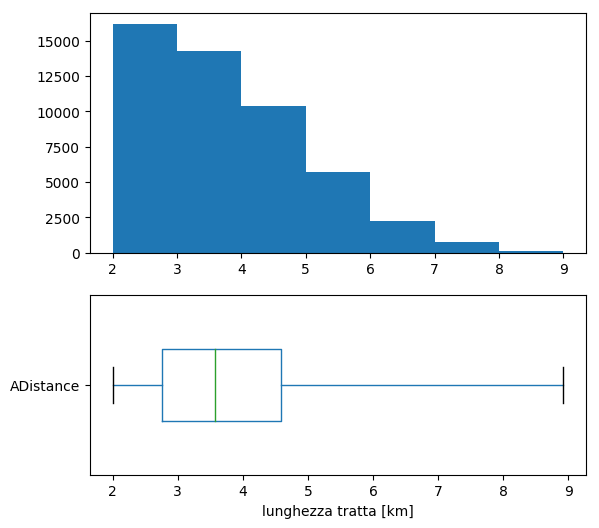
\includegraphics[scale=0.8]{distribuzione_tratte}
\end{center}

\begin{table}[H]
	\centering
	\begin{tabular}{ | l r | }
		\hline
		\textbf{Abs. freq.} & 49560 \\
		\textbf{media} & 3.80 \\
		\textbf{mediana} & 3.57 \\
		\textbf{std} & 1.27 \\
		\textbf{min} & 2.00 \\
		\textbf{max} & 9.52 \\
		\hline
	\end{tabular}
	\caption{Statistiche lunghezza tratta [km]}
	\label{table:2}
\end{table}

Nella tabella \ref{table:2} sono riportate le statistiche riguardo la lunghezza in via aerea delle tratte generate. Si può vedere come più della metà sia lunga meno di 5 km in linea aerea, risultato ottenuto in parte dai constraint imposti nella generazione.

\section{Performance medie}

\begin{table}[H]
	\centering
	\begin{tabular}{ | l r r r r r | }
		\hline
		& \textbf{Auto} & \textbf{Enjoy} & \textbf{ATM} & \textbf{Bici} & \textbf{Piedi} \\
		\textbf{media}   & 19.6 & 13.5 &  8.3 & 11.9 & 4.5 \\
		\textbf{mediana} & 19.5 & 13.2 &  7.9 & 12.0 & 4.5 \\
		\textbf{std}     &  3.9 &  3.8 &  2.3 &  1.3 & 0.0 \\
		\textbf{min}     &  6.7 &  3.0 &  3.4 &  6.5 & 4.3 \\
		\textbf{max}     & 48.5 & 36.1 & 27.8 & 16.9 & 4.6 \\
		\hline
	\end{tabular}
	\caption{Statistiche velocità media [km/h]}
	\label{table:3}
\end{table}

\section{Analisi dei singoli mezzi}




\subsection{Auto}

\subsubsection{Velocità media di ora in ora}

\begin{figure}[!h]
	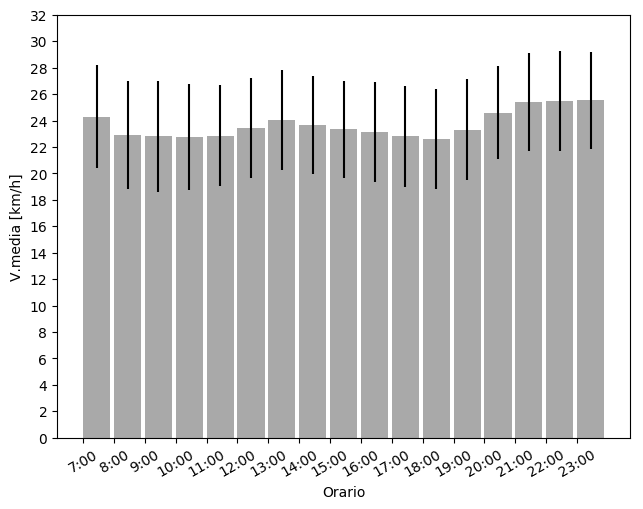
\includegraphics[scale=1.0]{vmedia_oraria_auto}
	\caption{Velocità media in auto [km/h] di ora in ora}
	\label{image:1}
\end{figure}

Una delle prime analisi effettuate per ogni mezzo è stata quella di calcolare la velocità media per ogni tragitto effettuato, con l'obbiettivo di osservare eventuali variazioni di ora in ora. Come riportato visualmente nella figura \ref{image:1}, i tragitti in macchina hanno subito una notevole variazione di velocità media nell'arco 8:00-11:00 e in quello delle 17:00-19:00. Tali risultati sono in linea con quelli dello studio di TomTomIndex\cite{tomtomindexmilan} effettuato sulla città di Milano nel 2019, che evidenzia le ore 9:00 e 18:00, anche dette \textit{rush hours}, come picchi di congestione stradale dal lunedì al venerdì, con un livello di congestione rispettivamente del 70\% e del 60\%. Risultano in linea con lo studio anche le ore precedenti e successive agli orari individuati come picchi.

\subsubsection{Velocità media lunedì-venerdì e sabato-domenica}

\begin{figure}[!h]
	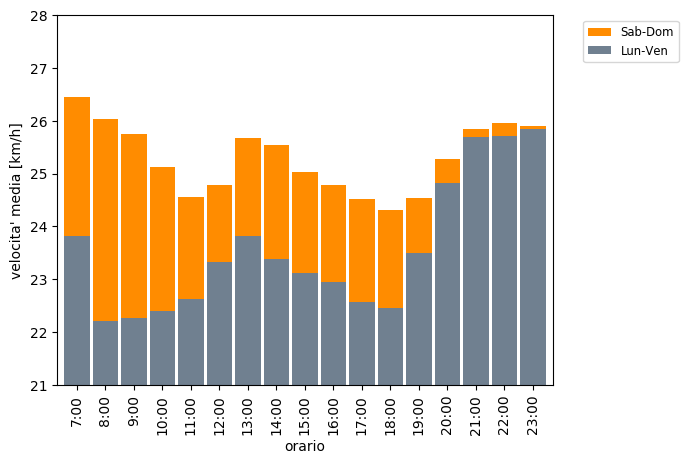
\includegraphics[scale=1.0]{vmedia_oraria_auto_weekend}
	\caption{Velocità media in auto [km/h] di ora in ora}
	\label{image:2}
\end{figure}

La figura \ref{image:2} mostra il risultato di una ripartizione dei dati effettuata sulla base del giorno della settimana, in particolare sono stati divisi i tragitti effettuati dal lunedì al venerdì di ogni settimana da quelli del sabato e domenica. Si può notare una notevole differenza di velocità media indistintamente dall'orario di circa 2 km/h. La variazione nel sabato-domenica risulta meno evidente di quella del lunedì-venerdì, con le variazioni, ovvero i picchi di rallentamento, che si spostanto nelle fasce orarie 10:00-12:00 e 16:00-19:00. Anche questi dati risultano in linea con quelli dello studio di TomTomIndex\cite{tomtomindexmilan}, che vede un minor livello di congestione nel weekend con dei picchi nelle ore 10:00 e 18:00.

\subsubsection{Velocità media settimana dopo settimana da fine lockdown}

\begin{figure}[!h]
	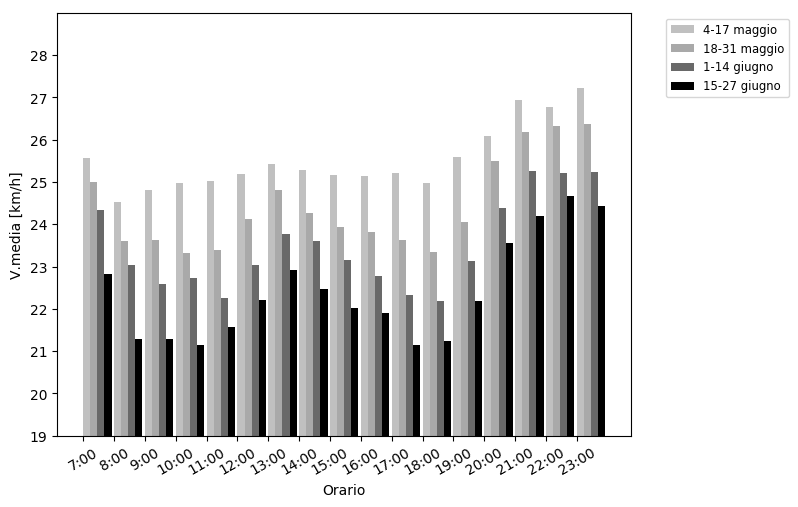
\includegraphics[scale=1.0]{vmedia_oraria_auto_weeks}
	\caption{Velocità media in auto [km/h] di ora in ora}
	\label{image:3}
\end{figure}



\subsection{Enjoy}

\begin{center}
	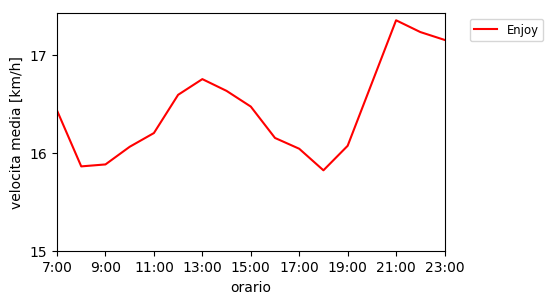
\includegraphics[scale=1.0]{vmedia_oraria_enjoy}
\end{center}

\begin{table}[H]
	\centering
	\begin{tabular}{ | l r | }
		\hline
		& \textbf{ragg. auto} \\
		\textbf{media}   &  6.6 \\
		\textbf{mediana} &  6.0 \\
		\textbf{std}     &  4.6 \\
		\textbf{min}     &  0.0 \\ 
		\textbf{max}     & 43.0 \\
		\hline
	\end{tabular}
	\caption{Statistiche t.medio per trovare auto [min]}
	\label{table:4}
\end{table}

\begin{center}
	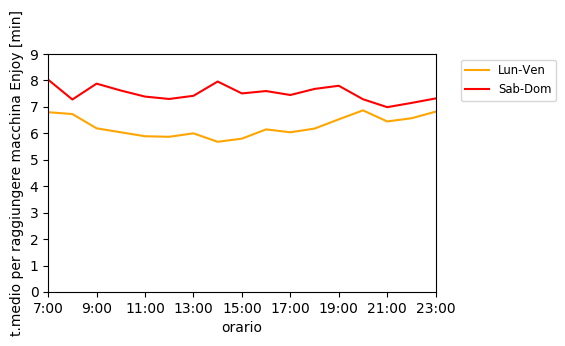
\includegraphics[scale=1.0]{tmedio_raggiungimento_auto_enjoy}
\end{center}

\begin{center}
	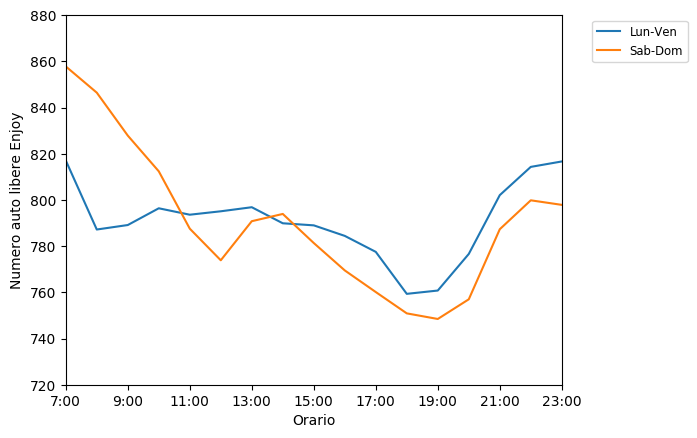
\includegraphics[scale=1.0]{variazione_auto_libere_enjoy_weekend}
\end{center}

\begin{center}
	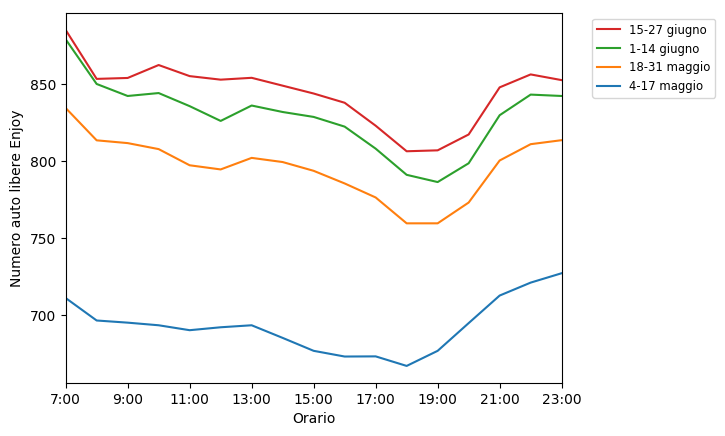
\includegraphics[scale=1.0]{variazione_auto_libere_enjoy_weeks}
\end{center}



\subsection{ATM, Bici e a piedi}

\begin{center}
	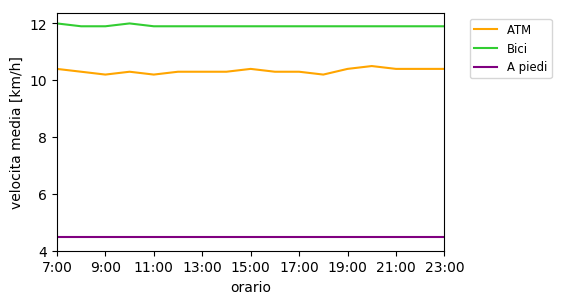
\includegraphics[scale=1.0]{vmedia_oraria_atm_bike_foot}
\end{center}


